
\documentclass[12]{article}
\usepackage[utf8]{inputenc}
\usepackage{cite}

\author{par4111 \\ Adrià Cabeza, Xavier Lacasa \\ Departament d' Arquitectura de Computadors}
\title{Lab 5: Geometric (data) decomposition: heat diffusion equation}
\date{\today \\ 2018 - 19 SPRING}
\usepackage{graphicx}
\usepackage{subcaption}
\usepackage{pgfplots}
\usepackage{listings}
\usepackage[margin=1.25in]{geometry}
\usepackage{xcolor}
\usepackage{float}
\lstset{
    language=C,
  basicstyle=\ttfamily,
  showstringspaces=false,
  commentstyle=\color{purple},
  keywordstyle=\color{blue},
	frame=tb,language=python,breaklines=true,numbers=none,  stringstyle=\color{red}, tabsize=3,   showstringspaces=false,
  columns=flexible, 
}
\pgfplotsset{compat=1.15}
\begin{document}
\maketitle

\vspace*{\fill}
\begin{center}

\includegraphics[scale=0.35]{images/UPClogo.png}
\end{center}
\newpage
\tableofcontents
\newpage
\section{Introduction}
In this laboratory session we will be dealing with a real problem and we will try to parallelize a piece of code using the most convenient task strategy. 
\\

All our different parallelization strategies will be made on a sequential code called \textit{heat.c}. This code simulates heat diffusion in a solid body using two different solvers for the heat equation: \textbf{Jacobi} and \textbf{Gauss-Seidel}.
\medskip

\begin{figure}[H]
\begin{subfigure}{.4\textwidth}
    \centering
    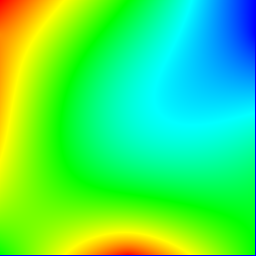
\includegraphics[scale=0.4]{images/heat-jacobi.png}
    \caption{Heat simulation using Jacobi}
\end{subfigure}
\begin{subfigure}{.4\textwidth}
    \centering
    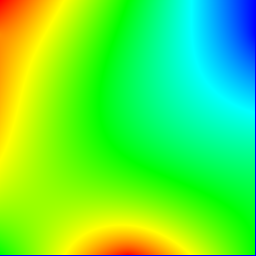
\includegraphics[scale=0.4]{images/heat-gauss.png}
    \caption{Heat simulation using Gauss}
\end{subfigure}
\end{figure}


\section{Analysis of task granularities and dependences}
In this section we will use \textit{Tareador} to analyse the task graphs generated when using the two different solvers. These dependency graphs will be really useful in order to implement the proper parallelization strategy.
\\

Firstly we have used Tareador to see the dependency graph of the versions that were already given, for the \textbf{Jacobi} and the \textbf{Gauss-Seidel} solvers.

\medskip

The parallelization strategy used for both solvers was to generate the finest grain tasks possible. To archieve it we have created a task inside the innermost loop of both methods.
\\
After implementing the previous strategy we checked the Tareador to see the dependency graph of each solver.

\begin{figure}[H]
\begin{subfigure}{.5\textwidth}
    \centering
    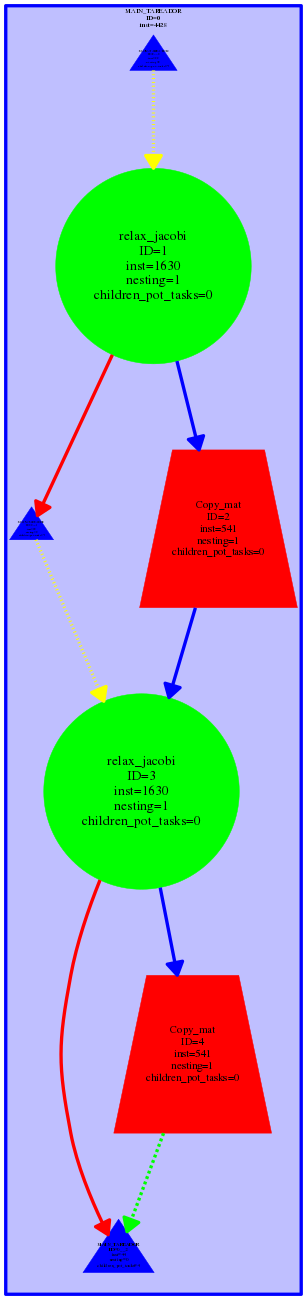
\includegraphics[scale=0.30]{images/jacobi.png}
    \caption{Jacobi dependencies}
\end{subfigure}
\begin{subfigure}{.5\textwidth}
    \centering
    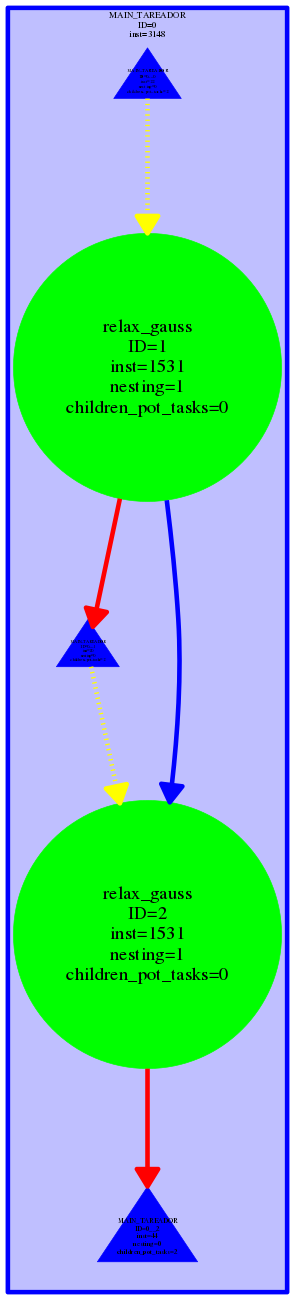
\includegraphics[scale=0.30]{images/gauss.png}
    \caption{Gauss-Seidel dependencies}
\end{subfigure}
\end{figure}


\subsection{Jacobi}
Code for the innermost loop parallelization strategy:
\medskip

\begin{lstlisting}[frame=single]
double relax_jacobi (double *u, double *utmp, unsigned sizex, unsigned sizey)
{
    double diff, sum=0.0;
  
    int howmany=4;
    for (int blockid = 0; blockid < howmany; ++blockid) {
      int i_start = lowerb(blockid, howmany, sizex);
      int i_end = upperb(blockid, howmany, sizex);
      for (int i=max(1, i_start); i<= min(sizex-2, i_end); i++) {
        for (int j=1; j<= sizey-2; j++) {
	     tareador_start_task("inner_loop_jacobi");
	     utmp[i*sizey+j]= 0.25 * ( u[ i*sizey     + (j-1) ]+  // left
	                               u[ i*sizey     + (j+1) ]+  // right
				       u[ (i-1)*sizey + j     ]+  // top
				       u[ (i+1)*sizey + j     ]); // bottom
	     diff = utmp[i*sizey+j] - u[i*sizey + j];
	     sum += diff * diff; 
	     tareador_end_task("inner_loop_jacobi");
	 }
      }
    }

    return sum;
}
\end{lstlisting}

\begin{figure}[H]
    \centering
    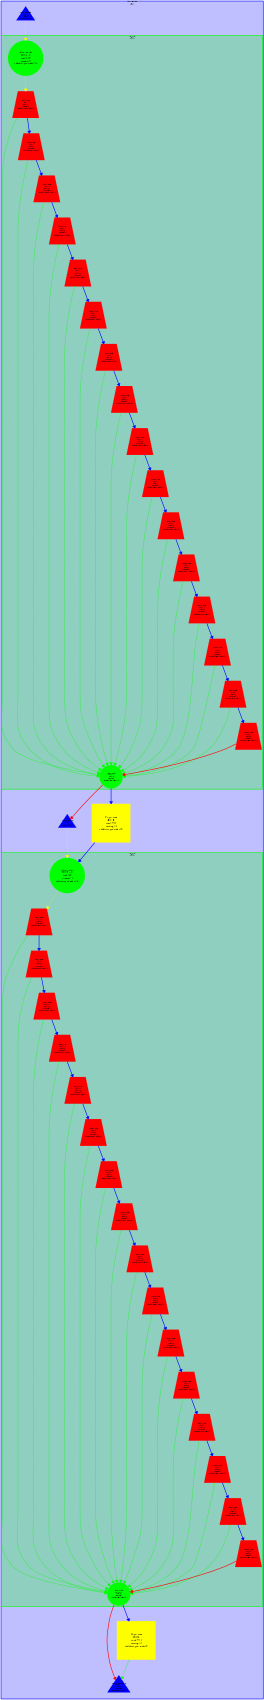
\includegraphics[scale=0.35]{images/dependency_jacobi.png}
    \caption{Dependency graph for Jacobi}
    \label{jacobi_dependency}
\end{figure}

We have observed that there is dependency over the sum variable: it is causing serialization of the tasks. If we ignore it from the analysis, please see figure \ref{code}, the dependency changes completely (see in Figure \ref{jacobi_dependency2} and we obtain a completely flat dependency graph, which means that the only dependence in the program was that variable.
\begin{figure}[H]
    \centering
    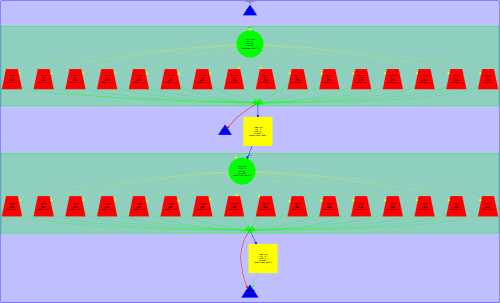
\includegraphics[scale=0.75]{images/dependency_jacobi2.png}
    \caption{Dependency graph for Jacobi without sum variable}
    \label{jacobi_dependency2}
\end{figure}

\begin{figure}[H]
\begin{lstlisting}[frame=single]
         ...
         tareador_disable_object(&sum);
         sum += diff * diff;
         tareador_enable_object(&sum);
        ...
\end{lstlisting}
\caption{Code snippet to disable the variable sum}
\label{code}
\end{figure}

\subsection{Gauss-Seidel}
Code for the innermost loop parallelization strategy:
\medskip

\begin{lstlisting}[frame=single]
double relax_gauss (double *u, unsigned sizex, unsigned sizey)
{
    double unew, diff, sum=0.0;

    int howmany=4;
    for (int blockid = 0; blockid < howmany; ++blockid) {
      int i_start = lowerb(blockid, howmany, sizex);
      int i_end = upperb(blockid, howmany, sizex);
      for (int i=max(1, i_start); i<= min(sizex-2, i_end); i++) {
        for (int j=1; j<= sizey-2; j++) {
	    tareador_start_task("inner_loop_gauss");
	    unew= 0.25 * ( u[ i*sizey	+ (j-1) ]+  // left
			   u[ i*sizey	+ (j+1) ]+  // right
			   u[ (i-1)*sizey	+ j     ]+  // top
			   u[ (i+1)*sizey	+ j     ]); // bottom
	    diff = unew - u[i*sizey+ j];
	    sum += diff * diff; 
	    u[i*sizey+j]=unew;
	    tareador_end_task("inner_loop_gauss");
        }
      }
    }
    return sum;
}
\end{lstlisting}

\begin{figure}[H]
    \centering
    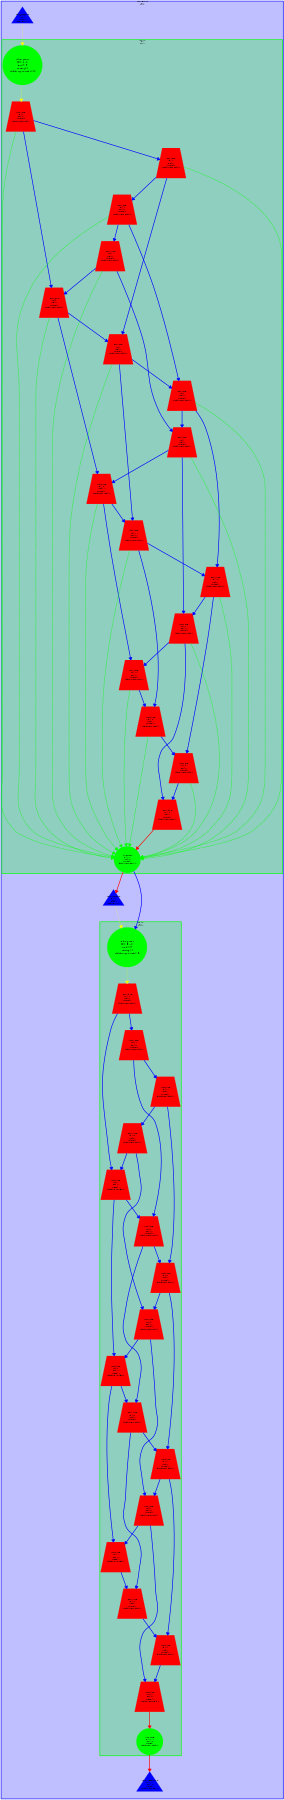
\includegraphics[scale=0.3]{images/dependency_gauss.png}
    \caption{Dependency graph for Gauss-Seidel}
    \label{Gauss_seidel_dependency}
\end{figure}

After implementing the innermost loop task stategy we have used \textit{Tareador} to see the dependency graph and we have observed some dependencies. Like in the previous version (Jacobi), we have disabled the sum variable (adding the piece of code in figure \ref{code}) to see if that variable was the only one provoking dependencies. However we can see that we still have dependencies (see \ref{Gauss_seidel_dependency2}). 

\begin{figure}[H]
    \centering
    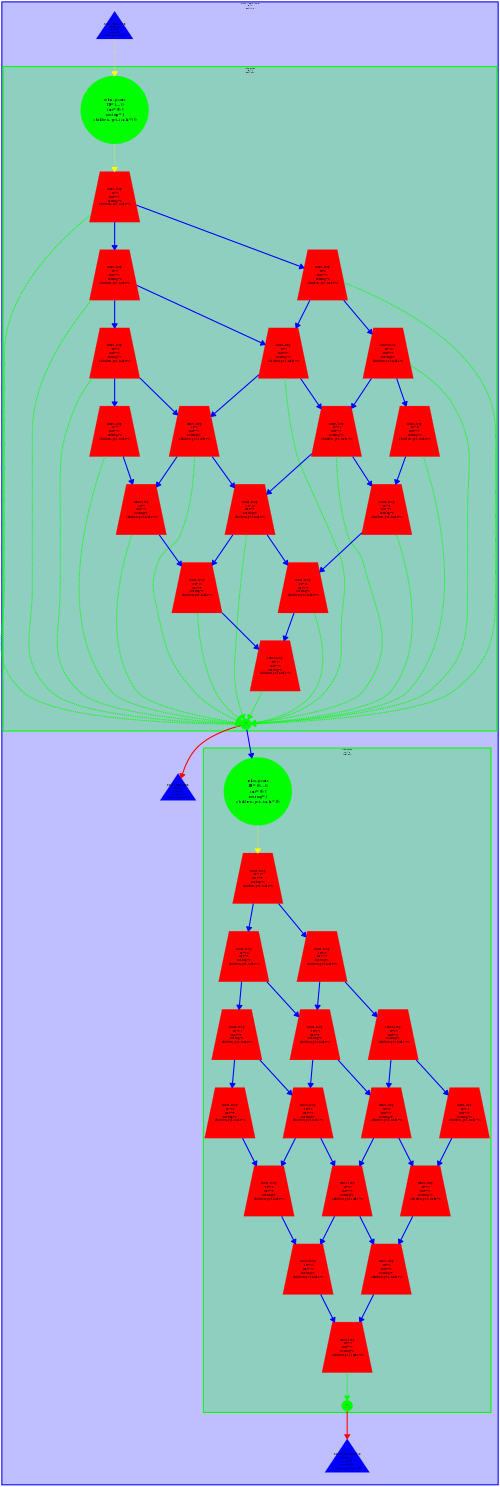
\includegraphics[scale=0.30]{images/dependency_gauss2.png}
    \caption{Dependency graph for Gauss-Seidel without variable sum}
    \label{Gauss_seidel_dependency2}
\end{figure}

If we had to guarantee these dependences using \textit{OpenMP} parallelization based on \textbf{\#pragma omp for} we would do it using a \textbf{reduction construct}. Using this construction we would be able to prevent sequential execution. This solution stores the partial results in a vector and after the parallel region makes the sum of the partial results of each threads. However several other techniques could have been applied like using a critical pragma combined with a shared variable sum, using a pragma atomic instead of critical, etc. 


\section{OpenMP parallelization and execution analysis: \textit{Jacobi}}

Based on the dependencies analysis we have already made, we will paralellize it using \textbf{\#pragma omp} constructions. However, we will not implement the maximum granularity because that would cause too much overhead. In order to solve it we must apply a data decomposition. First we have to choose between the input or output data structures that must be decomposed. Then, this structure will be partitioned across tasks following a data distribution: block, cyclic or block-cyclic.
\\

In this case the solution must group consecutive pixels, that is to say, use blocks; being $block\_size = n\_rows \div n\_threads$, so each thread does a block. With \textbf{Jacobi} we have a table of size \textit{N} and we divide N by the number of threads obtaining this:

\begin{figure}[H]
    \centering
    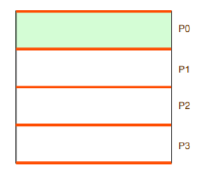
\includegraphics[scale=0.55]{images/geometric_jacobi.png}
    \caption{Jacobi data decomposition}
\end{figure}

Down below, you will find the code for the Jacobi implementation. We used \textbf{\#pragma omp parallel for} in the first loop. Moreover, as we said before, in order to solve the sum dependency, we will use a \textbf{reduction}. We have also noticed that the variable \textbf{diff} has dependencies, so we have solved it too.
\\
After implementing everything, we noticed that we had a serialization because of the matrix so we had to paralellize it too. 
\medskip

\begin{lstlisting}[frame=single]
/*
 * Function to copy one matrix into another
 */
void copy_mat (double *u, double *v, unsigned sizex, unsigned sizey)
{
    #pragma omp parallel for collapse(2) schedule(static,1)
    for (int i=1; i<=sizex-2; i++)
        for (int j=1; j<=sizey-2; j++)
            v[ i*sizey+j ] = u[ i*sizey+j ];
}

/*
 * Blocked Jacobi solver: one iteration step
 */
double relax_jacobi (double *u, double *utmp, unsigned sizex, unsigned sizey)
{
    double diff, sum=0.0;
    #pragma omp parallel private (diff) reduction(+: sum)
    {
    int blockid = omp_get_thread_num();
    int howmany=omp_get_num_threads();
    int i_start = lowerb(blockid, howmany, sizex);
    int i_end = upperb(blockid, howmany, sizex);
    for (int i=max(1, i_start); i<= min(sizex-2, i_end); i++) {
      for (int j=1; j<= sizey-2; j++) {
           
	   utmp[i*sizey+j]= 0.25 * ( u[ i*sizey     + (j-1) ]+  // left
	                             u[ i*sizey     + (j+1) ]+  // right
	                   	     u[ (i-1)*sizey + j     ]+  // top
				     u[ (i+1)*sizey + j     ]); // bottom
	   diff = utmp[i*sizey+j] - u[i*sizey + j];
	   sum += diff * diff; 
             	 
       }
    }
    }
    return sum;
}

\end{lstlisting}


Here we can see the scalability of two versions: the one that has not parallelized the \textit{copymat} function and the one we have given, which parallelizes everything:


%%AQUESTS PLOTS TOT I SER ELS QUE EM SURTEN NO TENEN PUTO SENTIT
\begin{center}
    \begin{figure}[H]
\begin{subfigure}{.5\textwidth}
    \centering
    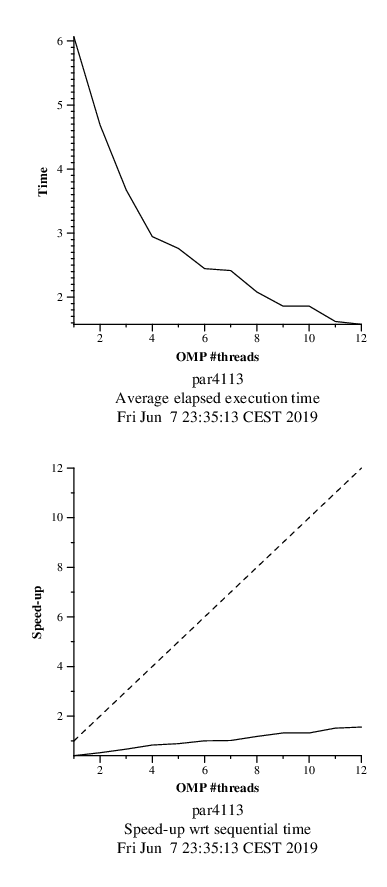
\includegraphics[scale=0.4]{images/nomatrixStrong.PNG}}
    \caption{Scalability plot for Jacobi without parallelizing the matrix}
    \label{copymat}
\end{subfigure}
\begin{subfigure}{.5\textwidth}
    \centering
    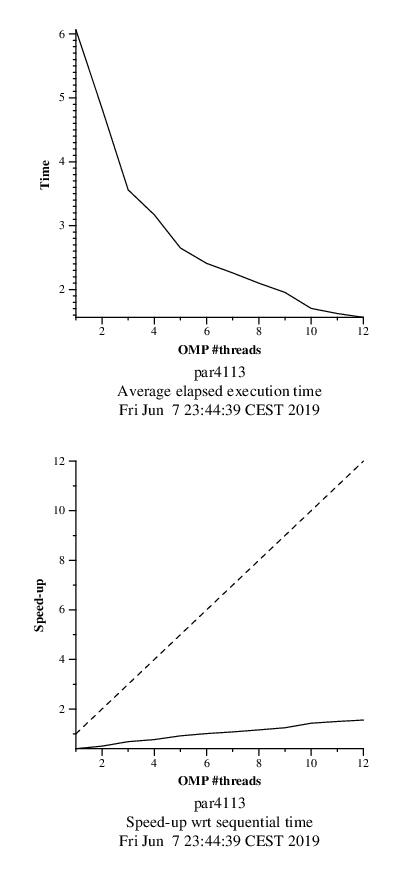
\includegraphics[scale=0.4]{images/matrixStrong.PNG}}
    \caption{Scalability plot for Jacobi}
    \label{scalability_jacobi}
\end{subfigure}
\end{figure}
\end{center}

We can see that the speed-up obtained with the Jacobi implementation improves while the number of threads executing the code is also increased. However when the ninth thtread is reached, the speed-up changes because of synchronization problems. Further parallelization analysis is shown in the respective Paraver traces:

\begin{center}
    \begin{figure}[H]
\begin{subfigure}{.5\textwidth}
    \centering
    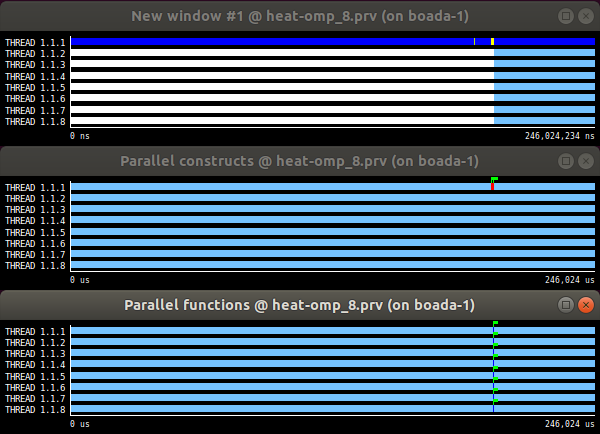
\includegraphics[scale=0.4]{images/nomatrixcopy.PNG}
    \caption{Paraver traces for Jacobi without parallelizing the matrix}
    \label{copymat}
\end{subfigure}
\begin{subfigure}{.5\textwidth}
    \centering
    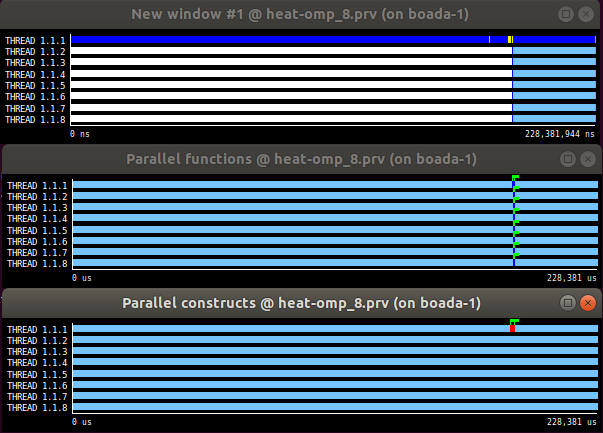
\includegraphics[scale=0.4]{images/matrixcopy.PNG}
    \caption{Paraver traces for Jacobi}
    \label{scalability_jacobi}
\end{subfigure}
\end{figure}
\end{center}


\section{OpenMP parallelization and execution analysis: \textit{Gauss-Seidel}}
In this section we are going to parallelize \textit{relax\_gauss}, in order to tranform the sequential execution into a parallel one. To do so, we have to do locking by column. Add a new loop and implement the synchronization of the blocks.
\medskip


\begin{lstlisting}[frame=single]
/*
 * Blocked Gauss-Seidel solver: one iteration step
 */
double relax_gauss (double *u, unsigned sizex, unsigned sizey)
{
    double unew, diff, sum=0.0;
    int howmany=4;

    #pragma omp parallel for ordered(2) private(unew, diff) reduction(+:sum)
    for (int blockid_row = 0; blockid_row < howmany; ++blockid_row) {
      for (int blockid_col = 0; blockid_col < howmany; ++blockid_col) {
        int i_start = lowerb(blockid_row, howmany, sizex);
        int i_end = upperb(blockid_row, howmany, sizex);
        int j_start = lowerb(blockid_col, howmany, sizey);
        int j_end = upperb(blockid_col, howmany, sizey);

        #pragma omp ordered depend (sink: blockid_row-1, blockid_col)
        for (int i=max(1, i_start); i<= min(sizex-2, i_end); i++) {
          for (int j=max(1, j_start); j<= min(sizey-2, j_end); j++) {
	    unew= 0.25 * ( u[ i*sizey	+ (j-1) ]+  // left
			   u[ i*sizey	+ (j+1) ]+  // right
			   u[ (i-1)*sizey	+ j     ]+  // top
			   u[ (i+1)*sizey	+ j     ]); // bottom
	     diff = unew - u[i*sizey+ j];
	     sum += diff * diff; 
	     u[i*sizey+j]=unew;
          }
        }
        #pragma omp ordered depend(source)
      }
    }
    return sum;
}

\end{lstlisting}

In the following plots, we can see the speed-up obtained with the Gauss-Seidel implementation varying the number of threads. We can see that the speed-up improves as the number of threads increase. However as it is seen in both plots it does not improve too much after 4 threads are reached. 

Here we can see the scalability plot
\begin{figure}[H]
    \centering
    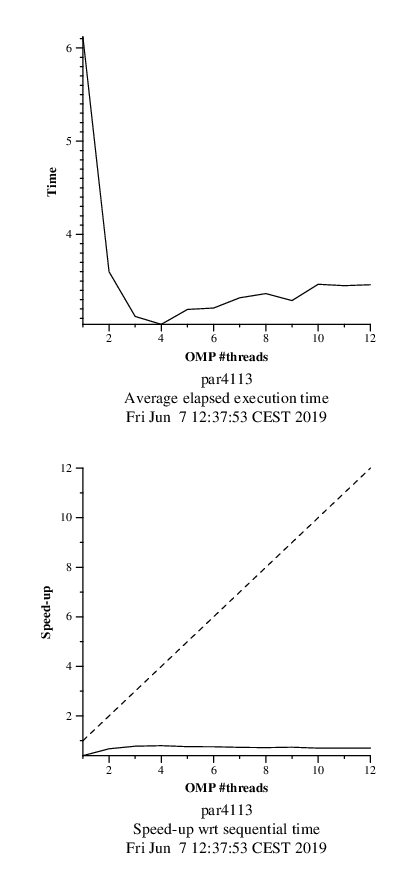
\includegraphics[scale=0.50]{images/heat-omp-strongGauss.PNG}
    \caption{Scalability plot for Gauss-Seidel}
    \label{scalability_gauss}
\end{figure}


As you may have noticed, parallelize the \textbf{Gauss-Seidel} function is more complicated than the Jacobi one. That is because we find dependencies between iterations and to solve it we have implemented a block distribution as opposed to the row decomposition we had initially implemented. By using this kind of decomposition we can avoid the dependency that was generated in the \textit{i-1} and \textit{j-1} elements. 

Paraver traces look as follow:
\begin{figure}[H]
    \centering
    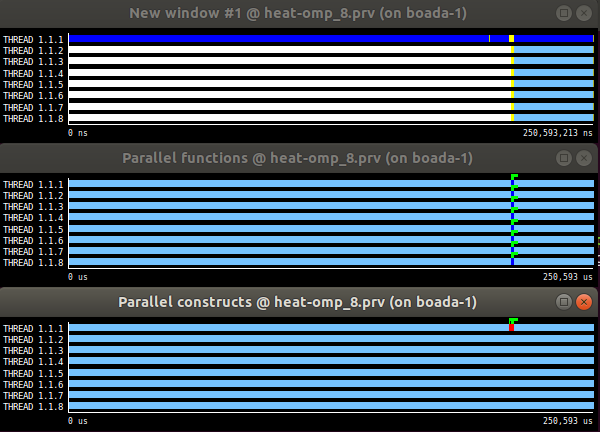
\includegraphics[scale=0.50]{images/gaussParaver.PNG}
    \caption{Paraver traces for Gauss-Seidel}
    \label{scalability_gauss}
\end{figure}

\section{Conclusion}
In this laboratory we have been able to parallelize a complex code of two equations solvers for a real world problem. We have also experimented what can happen in performance whenever there are dependencies and we learned to solve it.
\\

We can conclude that in the this subject we have learned from basic to more advanced concepts about parallelization using good and prepared material, like boada or paraver. It has been a good experience and we have learnt a lot in those laboratory sessions. 
\end{document}
